% id: 0542
% book: RPM 공통수학1 · 06 이차방정식과 이차함수
% section: 유형 UP 11 이차함수의 최대·최소의 활용
% figure: crop:fig-0542.png
% answer: $18\,\mathrm{m}$
% answer_source: 답지
% variant_level: 0 (원본 전사)
% 이 파일은 build.mjs 가 items.json 에서 만든다. 고칠 때는 items.json 을 고친다.
\smash{\raisebox{1.5mm}{\dmkichul{RPM 공통수학1 0542번 · 77쪽}}}
\noindent\begin{minipage}[t]{0.58\linewidth}\vspace{0pt}\raggedright 오른쪽 그림과 같이 밑변의 길이가 $10\,\mathrm{m}$, 높이가 $8\,\mathrm{m}$인 삼각형 모양의 땅에 내접하는 직사각형 모양의 밭을 만들려고 한다. 밭의 넓이가 최대일 때의 밭의 둘레의 길이를 구하시오.\end{minipage}\hfill\begin{minipage}[t]{0.4\linewidth}\vspace{0pt}\centering 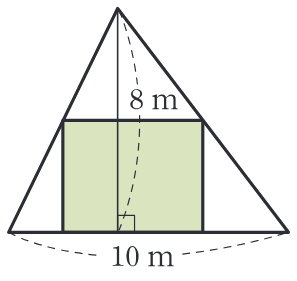
\includegraphics[width=71.2pt]{figures/fig-0542.png}\end{minipage}\par
